\section{方法学}
\label{sec:event}

在本节中，我们介绍了\textit{{O}n-{P}olicy {D}istillation with Tail {Res}idualization}（ResOPD）的理论基础与算法框架。  
我们在第~\ref{subsec:prelim}节中首先建立了全词表逆KL梯度，并分析了稀疏教师输出所引发的权衡问题，揭示了朴素的Top-$k$启发式方法如何导致目标偏差，以及为何混合估计量如HETS会受到尾部采样方差的影响。  
在第~\ref{subsec:cfr}节中，我们提出了ResOPD（如图~\ref{fig:framework}所示），展示了聚合尾部质量如何作为解析控制变量，以实现无偏且方差降低的估计量。  
第~\ref{subsec:evidence}节描述了采样假设，并将理论协方差界与可观测的在线诊断及下游任务性能联系起来。  
最后，第~\ref{sec:unified}节将分析扩展至双控制参数族。



\subsection{预备知识：从采样梯度到精确的稀疏头部}
\label{subsec:prelim}

在某一固定的轨迹前缀下，设 $p(i)>0$  和 $q(i)>0$ 表示学生模型和教师模型在共享词表 $\mathcal V$ 上的下一个 token 概率。定义
\begin{equation}
 \begin{aligned}
 r_i &\coloneqq \log\frac{p_i}{q_i}, &
 \bscore_i &\coloneqq \nabla_\theta\log p_i, &
 \btoken_i &\coloneqq r_i\bscore_i.
 \end{aligned}
 \label{eq:token-gradient}
\end{equation}
由于 $\sum_i p_i\bscore_i=\bm 0$ ，全词表反向KL梯度为
\begin{equation}
 \bgrad
 =\sum_i p_i\btoken_i
 =\E_{A\sim p}\!\left[\btoken_A\right].
 \label{eq:full-gradient}
\end{equation}
此处，$\btoken_A$ 表示停止系数采样 token 的 OPD 梯度。公式~(\ref{eq:full-gradient}) 表明，该采样 token 梯度是全词表反向 KL 梯度的无偏估计量。

\paragraph{为什么直接使用教师模型的 Top-$k$  rKL 会产生有偏结果。}
令 $S$ 为固定的教师 Top-$k$ 支持，其中 $0<k<|\mathcal V|$ ， $P=\sum_{i\in S}p_i$  和
$Q=\sum_{i\in S}q_i$ 。两种常见的标量快捷方式具有不同的偏差：
\begin{equation}
 L_{\mathrm{renormalized}}
 =\KL\!\left(\frac{p_S}{P}\middle\|\frac{q_S}{Q}\right),
 \qquad
 L_{\mathrm{truncated}}=\sum_{i\in S}p_i\log\frac{p_i}{q_i}.
 \label{eq:topk-shortcuts}
\end{equation}
重新规范化仅取决于 $S$ 内的条件分布。并且对于每个省略的 Logit $z_j$ ， $\partial L_{\mathrm{renormalized}}/\partial z_j=0$ 。截断保留了未规范化的头部但引入了一个边界项：
\begin{equation}
 \frac{\partial L_{\mathrm{truncated}}}{\partial z_j}
 =-p_j\underbrace{\sum_{i\in S}p_i(r_i+1)}_{C_S},
 \qquad j\notin S.
 \label{eq:truncated-tail-push}
\end{equation}
当 $C_S>0$ 时，梯度下降会增加每个被省略的 Logit。我们在实验中采用停止系数的替代方法 \citep{zhu2026many} $\bhead=\sum_{i\in S}p_i r_i\bscore_i$，这种方法避免了标量边界项，但仍受省略尾部的影响。附录~\ref{app:topk-bias} 证明了上述三个声明。

\begin{figure}[t]
\centering
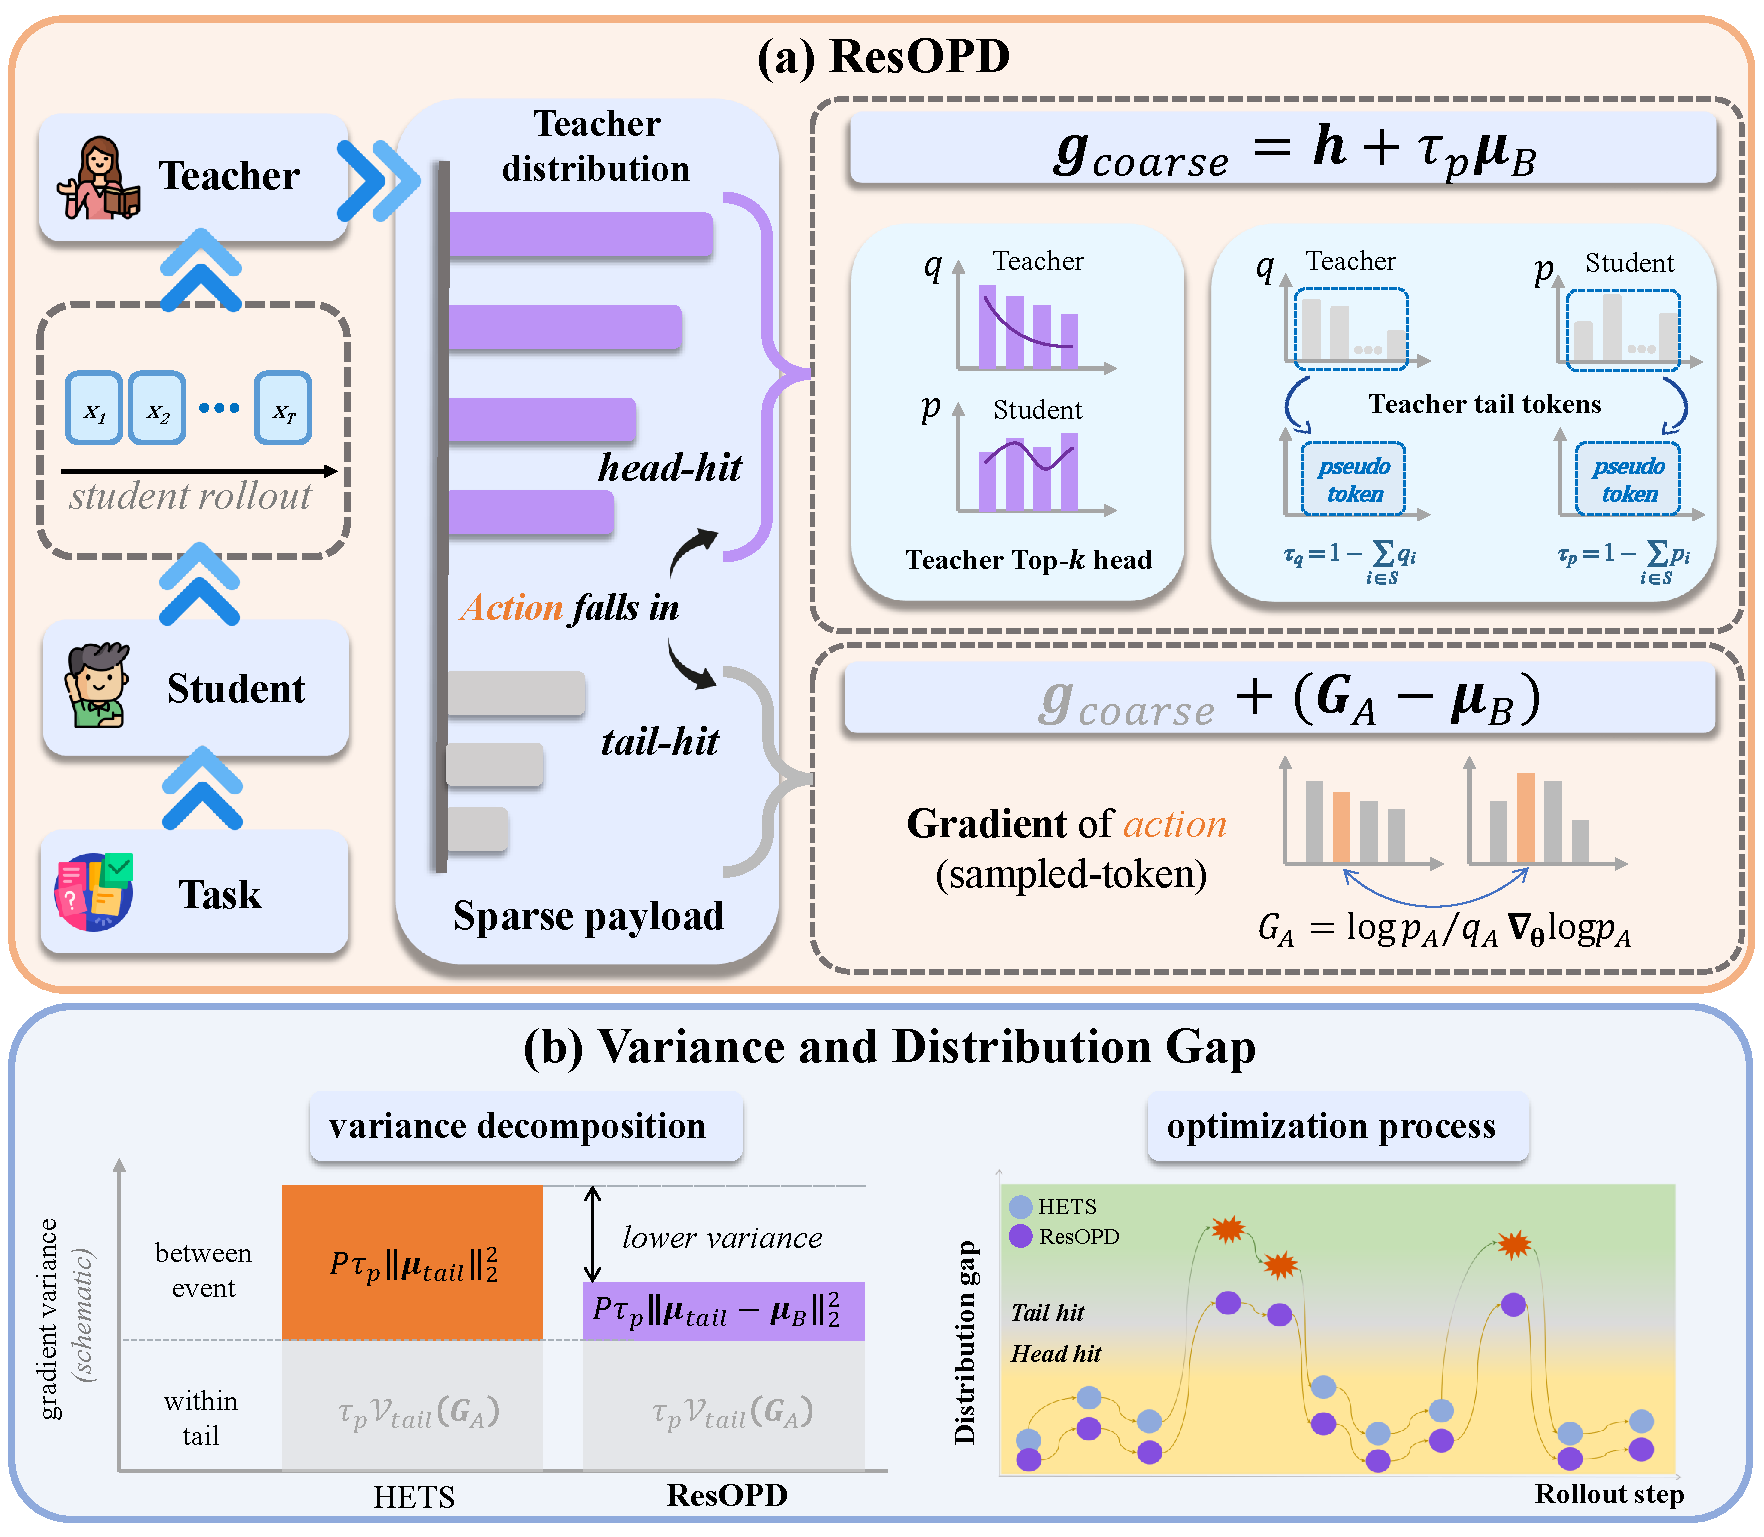
\includegraphics[width=0.8\textwidth]{figs/framework_v11.pdf}
\caption{
\textbf{ResOPD 概述。}
(a) 当学生样本 token 落在头部时，ResOPD 仅使用确切的粗粒度梯度；当命中尾部时，它添加残差修正。(b) 与 HETS 相比，ResOPD 通过将尾部样本集中在 $\boldsymbol{\mu}_B$ 附近，抑制了事件间的方差，从而在轨迹推进步骤中实现了与教师分布更优的对齐。
}
\label{fig:framework}
\end{figure}

接口返回 $q_i$  的完整规范化值以及 $i\in S$  和 $q_A$  的样本动作。
\begin{equation}
  \begin{gathered}
  \tau_p\coloneqq1-P,\qquad \tau_q\coloneqq1-Q,\\[-1pt]
  \bhead\coloneqq P\,\E[\btoken_A\mid A\in S] = \sum_{i\in S} p_i\btoken_i,
  \qquad
  \bmean_{\mathrm{tail}}\coloneqq
  \E\!\left[\btoken_A\mid A\notin S\right] = \frac{1}{\tau_p}\sum_{i\notin S} p_i\btoken_i.
  \end{gathered}
  \label{eq:head-tail-definitions}
\end{equation}
头部 $\bhead$ 是确切已知的，而细尾部平均梯度不可用。使用 $J=\ind\{A\notin S\}$ ，先验的头部确切尾部样本估计量为
\begin{equation}
 \widehat{\bgrad}^{\mathrm{HETS}}
 =\bhead+J\btoken_A,
 \qquad
 \E\!\left[\widehat{\bgrad}^{\mathrm{HETS}}\right]
 =\bhead+\tau_p\bmean_{\mathrm{tail}}=\bgrad.
 \label{eq:g0}
\end{equation}
在头部采样上，这个 \gzero{} 基准 \citep{zhang2026ema} 等于停止的教师 Top-$k$ rKL，并且仅在尾部采样上添加整个修正：
\begin{equation}
 \widehat{\bgrad}^{\mathrm{HETS}}
 =
 \begin{cases}
  \bhead, & A\in S,\\
  \bhead+\btoken_A, & A\notin S,
 \end{cases}
 \qquad
 \Pr(A\in S)=P.
 \label{eq:g0-rare-correction}
\end{equation}
大 $P$ 因此创建了一个稀疏修正模式：大多数 token 使用有偏的仅头部更新，而长小批量仍会累积大量采样的尾部修正。

\subsection{尾部残差化}
\label{subsec:cfr}

Top-$k$  also reveals aggregate tail masses.  
Following the tail-bucketing approach in \citet{hubotter2026reinforcement} and \citet{huang2026tail}, 将尾部合并为一个伪 token 可以得到
\begin{equation}
 \begin{aligned}
 b&\coloneqq\log\frac{\tau_p}{\tau_q}, &
 \bar{\bscore}_{\mathrm{tail}}
 &\coloneqq\E[\bscore_A\mid J=1]
   =\nabla_\theta\log\tau_p, &
 \bmean_B&\coloneqq b\,\bar{\bscore}_{\mathrm{tail}}.
 \end{aligned}
 \label{eq:bucket-vector}
\end{equation}
所得完整粗略分布的确切梯度是
\begin{equation}
 \bgrad_{\mathrm{coarse}}
 =\bhead+\tau_p\bmean_B.
 \label{eq:coarse-gradient}
\end{equation}
此处 $\bmean_B$ 作出预测，但不必等于不可用的细尾均值。事实上，此公式可泛化至任意基准向量：对于 $A\sim p$ 以及任意依赖前缀的基准向量 $\bcontrol$ ，
\begin{equation}
\widehat{\bgrad}(\bcontrol)=\bhead+\tau_p\bcontrol+J(\btoken_A-\bcontrol),
\label{eq:residualization}
\end{equation}
是无偏的，即 $\E_{A\sim p}\!\left[\widehat{\bgrad}(\bcontrol)\right]=\bgrad$ 。图~\ref{fig:framework} 总结了构造过程。HETS 是特殊情况 $\bcontrol=\bm0$ 。期望是显式的：
\begin{equation}
 \E[\widehat{\bgrad}(\bcontrol)]
 =\bhead+\tau_p\bcontrol
  +\tau_p(\bmean_{\mathrm{tail}}-\bcontrol)
 =\bgrad.
 \label{eq:residualization-expectation}
\end{equation}
该控制可能依赖于固定的前缀和当前的模型概率，但必须相对于采样的动作固定，并在反向传播之前停止。此外，将任意随机向量 $\bm{X}$ 的总方差定义为 $\mathcal{V}(\bm{X}) \coloneqq \operatorname{tr}(\operatorname{Cov}(\bm{X}))$，应用全协方差法则可得 $\widehat{\bgrad}(\bm B)$ 的显式方差：
\begin{equation}
\mathcal{V}(\widehat{\bgrad}(\bm B)) = \tau_p\mathcal{V}_{\mathrm{tail}}(\btoken_A)
+ P\tau_p\lVert\bmean_{\mathrm{tail}}-\bm B\rVert_2^2,
\label{eq:single-control-variance-1}
\end{equation}
其中 $\mathcal{V}_{\mathrm{tail}}(\btoken_A) \coloneqq \operatorname{tr}(\operatorname{Cov}(\btoken_A \mid A \in \mathrm{tail}))$。
此处，第一项 $\tau_p\mathcal{V}_{\mathrm{tail}}(\btoken_A)$ 捕捉了尾部采样方差的基准不变性（按尾部概率 $\tau_p$ 加权），而第二项则考虑了由残差近似误差 $\lVert\bmean_{\mathrm{tail}}-\bm B\rVert_2^2$ 引起的事件间方差，该方差通过 \(P\tau_p\)（头部与尾部指示变量的方差）进行缩放。
直接观察可知，对 $J$ 进行条件化：头部分支是确定性的，尾部分支保留 $\Cov_{\mathrm{tail}}(\btoken_A)$，且两者条件均值之差为 $\bmean_{\mathrm{tail}}-\bm B$。根据全协方差定律，得到公式~(\ref{eq:single-control-variance-1})。

公式~(\ref{eq:single-control-variance-1}) 还表明，当控制向量设置为真实的尾部均值时，即 $\bcontrol = \bmean_{\mathrm{tail}}$，估计量 $\widehat{\bgrad}(\bcontrol)$ 的方差达到最小。然而，在实际应用中 $\bmean_{\mathrm{tail}}$ 无法获得，因此 ResOPD 使用可计算的尾部分桶替代量 $\bmean_B$ 来代替它：
\begin{equation}
\widehat{\bgrad}^{\mathrm{ResOPD}}
=\bgrad_{\mathrm{coarse}}+J(\btoken_A-\bmean_B).
\label{eq:event}
\end{equation}

可预测的粗略修正现在每次绘制都会出现；只有细微尾部残差仍然罕见。当 $\lVert\bmean_{\mathrm{tail}}-\bmean_B\rVert_2 < \lVert\bmean_{\mathrm{tail}}\rVert_2$ 时，ResOPD 的方差严格低于 HETS，即当尾部桶向量 $\bmean_B$ 对真实尾部均值的预测优于零时，这在我们冻结前缀审计的总体观察中已得到验证。完整的推导过程见附录~\ref{app:single-control}。





\subsection{采样假设与证据边界}
\label{subsec:evidence}

上述无偏性恒等式假设在固定前缀处 $A\sim p_\theta$。滚动采样过滤器改变了这一采样规律。我们的主要数学实验（第~\ref{sec:math-opd}节）使用温度 $1.0$、滚动 top-$p=0.95$ 和滚动 top-$k=20$，而全支持审计（第~\ref{sec:exact-audit}节）和跨领域实验（第~\ref{sec:cross-domain}节）则采用祖先条件。第~\ref{sec:ex-setup}节同时指定了两者，第~\ref{sec:rollout-ablation}节评估移除过滤器的影响。

粗粒度到细粒度的方差分解也可以在任意实现的滚动分布 $\tilde p$ 下进行刻画。令 $\tilde{\tau}=\Pr_{\tilde p}(A\notin S)$ 和 $\tilde{\bm\mu}_{\mathrm{tail}}
=\mathbb{E}_{\tilde p}[\bm G_A\mid A\notin S]$。对于 $\hat{\bm g}(\bm B)=\bm h+\tau_p\bm B+
\mathbb{I}\{A\notin S\}(\bm G_A-\bm B)$，该估计量仍然具有确切的分解。
\begin{equation}
\mathcal V_{\tilde p}(\hat{\bm g}(\bm B))
=
\tilde{\tau}\mathcal V_{\tilde p,\mathrm{tail}}(\bm G_A)
+
(1-\tilde{\tau})\tilde{\tau}
\|\tilde{\bm\mu}_{\mathrm{tail}}-\bm B\|_2^2 .
\label{eq:realized-rollout-variance}
\end{equation}
因此，对于 $0<\tilde{\tau}<1$ ，当满足 $\|\tilde{\bm\mu}_{\mathrm{tail}}-\bm\mu_B\|_2
<\|\tilde{\bm\mu}_{\mathrm{tail}}\|_2$ 时，ResOPD 的采样方差严格低于 HETS。
在此实现的采样定律下的期望更新为
\begin{equation}
 \E_{\tilde p}[\widehat{\bgrad}(\bm B)]
 =\bhead+\tau_p\bm B
  +\tilde\tau(\tilde{\bm\mu}_{\mathrm{tail}}-\bm B).
 \label{eq:realized-rollout-mean}
\end{equation}
方差恒等式在 $\tilde p$ 下仍然确切成立，但它并不能将截断的滚动序列转化为从 $p_\theta$ 中无偏抽取的样本。  
关键的是，截断严格局限于序列生成过程。在训练期间，所有学生量（$p_i$、$r_i$、$s_i$、$\tau_p$ 以及粗尾项）均通过一次全新的、未截断的前向传播被准确重新计算。

公式~(\ref{eq:single-control-variance-1}) 在固定前缀下刻画了估计量的质量。我们通过确切的动作枚举进行测试（第~\ref{sec:exact-audit}~节）。在在线 OPD 过程中，策略和访问过的前缀均发生变化，而稀疏的教师反馈掩盖了尾部的细微信息。我们转而监控残差的二阶矩 \(M_2\)，作为一种低成本且与机制对齐的在线诊断手段。其下降趋势与头部与尾部事件噪声的减少一致，但本身并不能估计完整的梯度协方差。附录~\ref{app:online-residual-moments} 给出了确切的定义。

然而，方差减小并不意味着下游准确率的单调提升。降低协方差迹可以减少随机优化噪声，但最终性能仍受训练动态和解码随机性的影响，而这两者均通过基准评分进行了离散化。因此，ResOPD能够可靠地抑制梯度噪声，而无需在每个检查点都严格优于HETS。我们因此将理论协方差、在线残差矩以及下游准确率视为学习流水线不同阶段的互补信号。
